%%%%%%%%%%%%%%%%%%%%%%%%%%%%%%%%%%%%%%%%%
% Beamer Presentation
% LaTeX Template
% Version 1.0 (10/11/12)
%
% This template has been downloaded from:
% http://www.LaTeXTemplates.com
%
% License:
% CC BY-NC-SA 3.0 (http://creativecommons.org/licenses/by-nc-sa/3.0/)
%
%%%%%%%%%%%%%%%%%%%%%%%%%%%%%%%%%%%%%%%%%

%----------------------------------------------------------------------------------------
%	PACKAGES AND THEMES
%----------------------------------------------------------------------------------------

\documentclass{beamer}

\mode<presentation> {

% The Beamer class comes with a number of default slide themes
% which change the colors and layouts of slides. Below this is a list
% of all the themes, uncomment each in turn to see what they look like.

%\usetheme{default}
%\usetheme{AnnArbor}
%\usetheme{Antibes}
%\usetheme{Bergen}
%\usetheme{Berkeley}
%\usetheme{Berlin}
%\usetheme{Boadilla}
%\usetheme{CambridgeUS}
%\usetheme{Copenhagen}
%\usetheme{Darmstadt}
%\usetheme{Dresden}
%\usetheme{Frankfurt}
%\usetheme{Goettingen}
%\usetheme{Hannover}
%\usetheme{Ilmenau}
%\usetheme{JuanLesPins}
%\usetheme{Luebeck}
%\usetheme{Madrid}
%\usetheme{Malmoe}
%\usetheme{Marburg}
%\usetheme{Montpellier}
%\usetheme{PaloAlto}
%\usetheme{Pittsburgh}
%\usetheme{Rochester}
%\usetheme{Singapore}
%\usetheme{Szeged}
\usetheme{Warsaw}

% As well as themes, the Beamer class has a number of color themes
% for any slide theme. Uncomment each of these in turn to see how it
% changes the colors of your current slide theme.

%\usecolortheme{albatross}
%\usecolortheme{beaver}
%\usecolortheme{beetle}
%\usecolortheme{crane}
%\usecolortheme{dolphin}
%\usecolortheme{dove}
%\usecolortheme{fly}
%\usecolortheme{lily}
%\usecolortheme{orchid}
%\usecolortheme{rose}
%\usecolortheme{seagull}
%\usecolortheme{seahorse}
%\usecolortheme{whale}
%\usecolortheme{wolverine}

%\usepackage[utf8]{inputenc}

%\setbeamertemplate{footline} % To remove the footer line in all slides uncomment this line
%\setbeamertemplate{footline}[page number] % To replace the footer line in all slides with a simple slide count uncomment this line

%\setbeamertemplate{navigation symbols}{} % To remove the navigation symbols from the bottom of all slides uncomment this line
}

\usepackage{graphicx} % Allows including images
\usepackage{booktabs} % Allows the use of \toprule, \midrule and \bottomrule in tables
\usepackage{multicol}
\usepackage{amsmath}

\DeclareMathOperator{\argmin}{argmin} % no space, limits on side in displays


%----------------------------------------------------------------------------------------
%	TITLE PAGE
%----------------------------------------------------------------------------------------

\title[Face Recognition via Sparse Representation]{Face Recognition via Sparse Representation} % The short title appears at the bottom of every slide, the full title is only on the title page

\author{ Wabartha -  Durand -  Darmet -  Vayer} % Your name

\date{\today} % Date, can be changed to a custom date

\begin{document}

\begin{frame}
\titlepage % Print the title page as the first slide
\end{frame}

\begin{frame}
\frametitle{Overview} % Table of contents slide, comment this block out to remove it
  \tableofcontents
\end{frame}



%----------------------------------------------------------------------------------------
%	PRESENTATION SLIDES
%----------------------------------------------------------------------------------------
%------------------------------------------------
%------------------------------------------------

\AtBeginSection[]
  {
    \ifnum \value{framenumber}>1
      \begin{frame}<beamer>
      \frametitle{Plan}
      \tableofcontents[currentsection]
      \end{frame}
    \else
    \fi
  }
  
\section{Document presentation}

%------------------------------------------------

	\subsection{Article's origins}
	
	\begin{frame}
		\frametitle{Article's origins}

\begin{itemize}		
\item University of Illinois
\item PHD work of John Wright. Work on Face and object recognition. Student Member of IEEE. 16405 citations since 2012. Now work for Columbia University
\item Published in : IEEE transactions on pattern analysis and machine intelligence (TPMAI) in 2009 (a reference specialised in computer vision and patter analysis/recognition)
-\item Article cited by 6386 since 2009
-\item IEEE stand for Institute of Electrical and Electronics Engineers : almost a monopoly in the area. They organise enowned conferences.  
-\item J.Wright worked under the supervision of notably Yi Ma (a reference in Computer Vision)
\end{itemize}


	
			\end{frame}

%------------------------------------------------
			
	\subsection{Contributions}

	
	\begin{frame}
		\frametitle{Contributions}	
		

The main contribution of the article is concerning the sparse approach for image processing which leads to :
 	\begin{itemize}	
 	\item features extraction (eigenfaces,FisherFaces,...) is not crucial anymore 
 	\item occlusion, corruption and noises robust
 	\item fast (light computation)
 	\item Sparsity Concentration Index (efficently detect invalid images)	
	\end{itemize}
	
	\end{frame}
	
%------------------------------------------------


%------------------------------------------------
%------------------------------------------------
\section{Face recognition via Sparse representation}

	\subsection{Face recognition}
	
%------------------------------------------------
	
\begin{frame}
\frametitle{Face recognition}
			\begin{figure}[!ht]
			\begin{center}
			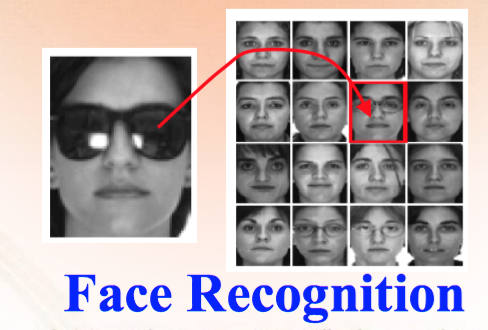
\includegraphics[scale=0.7]{face_recog.png}
			\end{center}
			\caption{Face recognition}
			\label{fa}
			\end{figure}
			

\end{frame}

\begin{frame}
\frametitle{Face recognition : our example}

			\begin{figure}[!ht]
			\begin{center}
			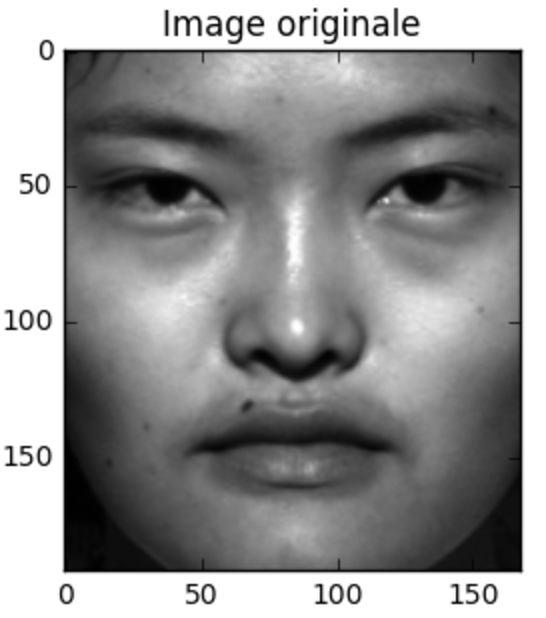
\includegraphics[scale=0.5]{original.png}
			\end{center}
			\caption{Face recognition}
			\label{fa}
			\end{figure}
\end{frame}
%------------------------------------------------

	\subsection{Sparse representation}
		
	
		\begin{frame}
		\frametitle{Symbols}
		
			\begin{itemize}
				\item Let's consider $k$ distinct object classes in the training data (k faces)
				\item An image of size $w \times h$  is indentified as a vector $v \in \mathbb{R}^{m}$ where $m=wh$ given by stacking it columns
				\item The $n_{i}$ given training samples, taken from the i-th class (face) are arranged as columns of a matrix $A_{i}=\lbrack v_{i,1},v_{i,2},...,v_{i,n_{i}} \rbrack \in \mathbb{R}^{m \times n_{i}} $
				\item So the columns of $A_{i}$ are the training face images of the i-th subject
				
			\end{itemize}

		\end{frame}

%------------------------------------------------

	
	\subsection{Mathematical related problem}
	
	%------------------------------------------------
	
		\begin{frame}
		\frametitle{Sparse Linear Combination}

Given some training samples of the i-th object class, $A_{i}=\lbrack v_{i,1},v_{i,2},...,v_{i,n_{i}} \rbrack \in \mathbb{R}^{m \times n_{i}} $, any new test sample $y \in \mathbb{R}^{m}$ \textbf{from the same class} will be described as as linear combination of the training samples associated with object i :

$$y=\alpha_{i,1}v_{i,1}+\alpha_{i,2}v_{i,2}+...+\alpha_{i,n_{i}}v_{i,n_{i}}$$

for some scalars $\alpha_{i,j} \in \mathbb{R}$

		\end{frame}
%------------------------------------------------

		\begin{frame}
		\frametitle{Sparse Linear Combination}

Since the membership i of a test sample is unknown we define a new matrix A as the concatenation of $n$ training samples of all $k$ object classes :

$$A=\lbrack A_{1},A_{2},...,A_{k} \rbrack $$

Such that the linear representation of $y$ can be written :

$$y=Ax_{0}  \in \mathbb{R}^{m} $$
where 
$$x_{0}=\lbrack 0,....,0,\alpha_{i,1},\alpha_{i,2},...,\alpha_{i,n_{i}},0,...,0  \rbrack \in \mathbb{R}^{m}$$


		\end{frame}

%------------------------------------------------
		
\begin{frame}

		\frametitle{Sparse Linear Combination}		
			
			\begin{figure}[!ht]
			\begin{center}
			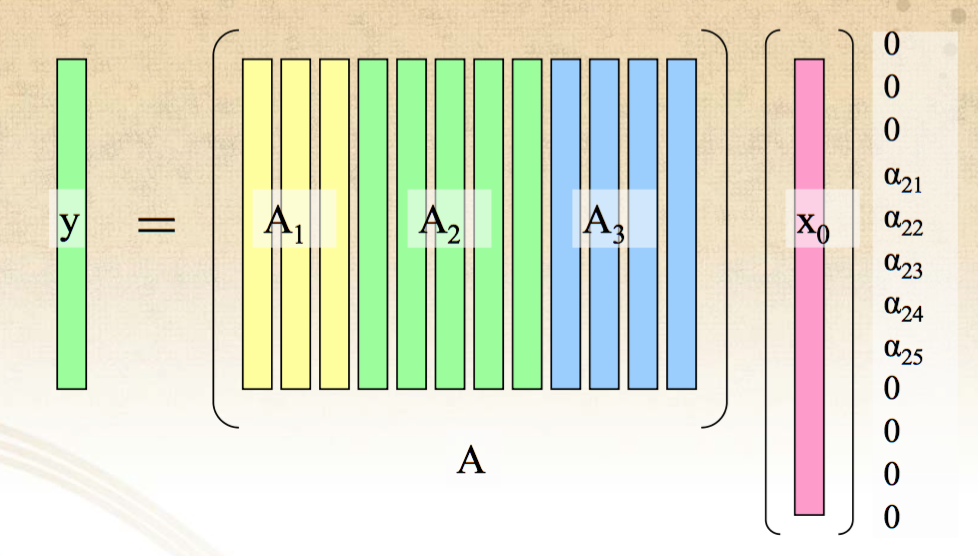
\includegraphics[scale=0.5]{sparse.png}
			\end{center}
			\caption{Sparse Linear Representation}
			\label{ma}
			\end{figure}

\end{frame}

%------------------------------------------------
		
\begin{frame}

		\frametitle{To solve $y=Ax$ via $L^{0}$}		
			
\begin{itemize}
\item The idea is \textbf{to seek the sparsest solution} to $y=AX$
\item Method :
	\begin{itemize}
	\item We can do it by solving : 
	$$ \hat{x_{0}}= \argmin \|x\|_{0}  \mbox{ subject to } Ax=y$$
	\item Where $\|.\|_{0} $is the $L^{0}$ norm which is the number of nonzero entries in a vector
	\end{itemize}
\item Problem : this problem is NP-hard, and difficult even to approximate (combinatorial optimization)


\end{itemize}

\end{frame}
%------------------------------------------------
		
\begin{frame}

		\frametitle{Sparse solution via  $L^{1}$ minimization}		
			
\begin{itemize}
\item Some results in the theory of sparse representation show that if the solution \textbf{$x_{0}$ is sparse enough} the solution to the problem above is equal to the solution of the $L^{1 }$ minimization problem :
	$$ \hat{x_{1}}= \argmin \|x\|_{1}  \mbox{ subject to } Ax=y$$
	
\item This problem can be solved in \textbf{polynomial time} by standard linear programming method

\end{itemize}

\end{frame}



%------------------------------------------------
		
\begin{frame}

		\frametitle{The main result}		
			
\begin{block}{Sparse solution for $L^{0}$ minimization via $L^{1}$}

As long as the number of nonzero entries of $x_{0}$ is a small fraction of the dimension m, $L^{1}$ minimization will recover $x_{0}$ 

\end{block}

			\begin{figure}[!ht]
			\begin{center}
			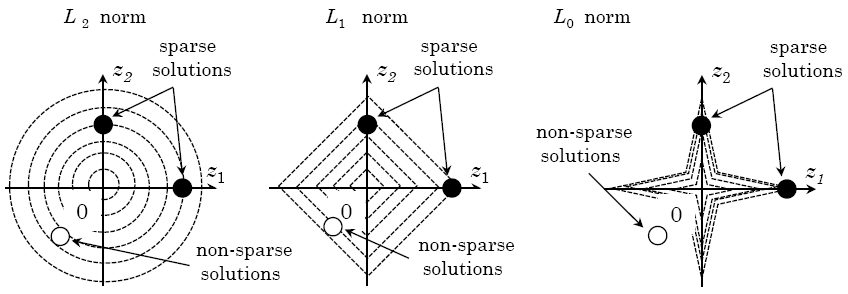
\includegraphics[scale=0.45]{sparse_sol.png}
			\end{center}
			\caption{Sparse solution}
			\label{fa}
			\end{figure}

\end{frame}

%------------------------------------------------	

\begin{frame}
\frametitle{Face recognition : our example}

			\begin{figure}[!ht]
			\begin{center}
			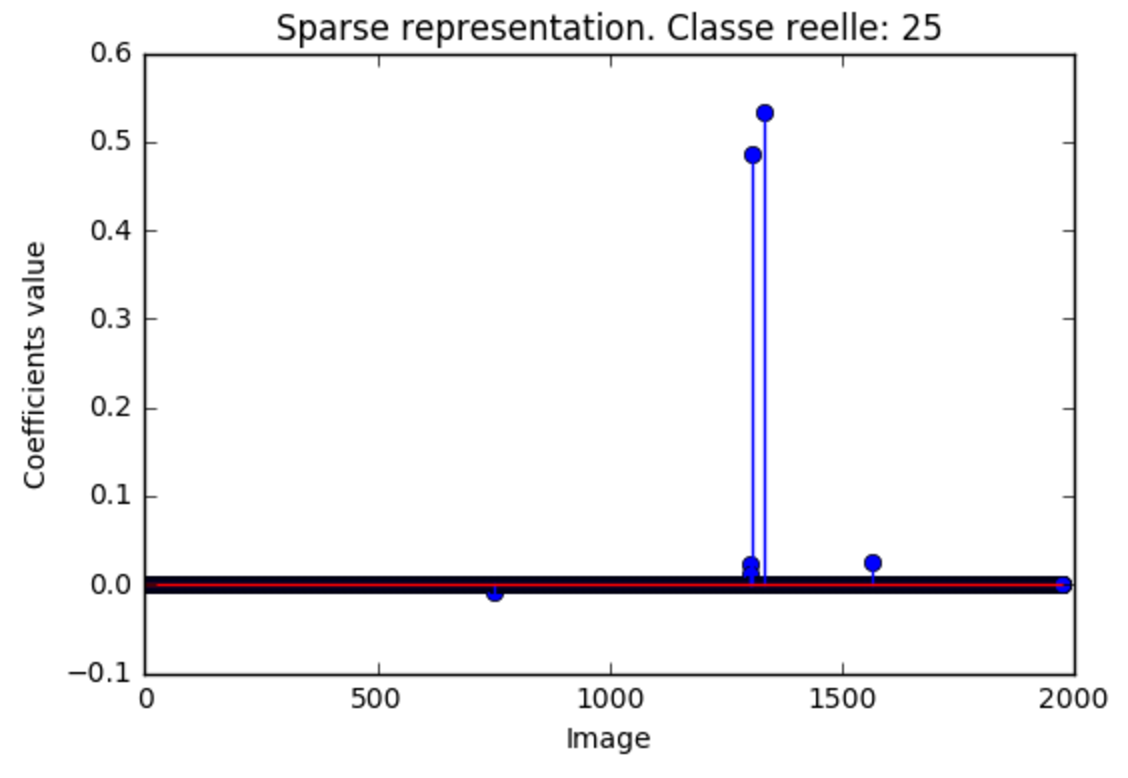
\includegraphics[scale=0.5]{sparsity.png}
			\end{center}
			\caption{Face recognition}
			\label{fa}
			\end{figure}
\end{frame}

%------------------------------------------------	
%------------------------------------------------
\section{Classification via Sparse representation}

	%------------------------------------------------
\subsection{Initial problem}

\begin{frame}

\frametitle{Methods}


	\begin{itemize}
	
\item For each class $i$, we denote $\delta_{i} : \mathbb{R}^{n} \to \mathbb{R}^{n}$ the characteristic function which selects the coefficients associated with the i-th class

\item Using only the coefficients associated with the i-th class, we can approximate the test sample $y$ as $\hat{y_{i}}=A\delta_{i}(\hat{x_{1}})$
\item We classify y based on the approximation that minimizes the residual $\|y-A\delta_{i}(\hat{x_{1}})\|_{2}$

	\end{itemize}

\end{frame}

%------------------------------------------------

\begin{frame}


\frametitle{Algorithm 1: Sparse representation based Classification (SRC)}		
			
\begin{block}{SRC}

	\begin{enumerate}
	
	\item Input : a matrix of training samples $A=\lbrack A_{1},A_{2},...,A_{k} \rbrack \in \mathbb{R}^{m \times n}$ for k classes and a test sample $y \in \mathbb{R}^{m}$
	\item Normalize the columns of A to have unit $L^{2}$ norm
	\item Solve the $L^{1}$ minimization problem :
		$$ \hat{x_{1}}= \argmin \|x\|_{1}  \mbox{ subject to } Ax=y$$
		
	\item Compute the residuals
	$ \mbox{ for all } i=1,...k, r_{i}(y)=\|y-A\delta_{i}(\hat{x_{1}})\|_{2}$
	
	\item $\mathcal{C}_{y}=\argmin_{i} r_{i}(y)$
	
	
	\end{enumerate}



\end{block}

\end{frame}

%---------------

\begin{frame}
\frametitle{Face recognition : our example}

			\begin{figure}[!ht]
			\begin{center}
			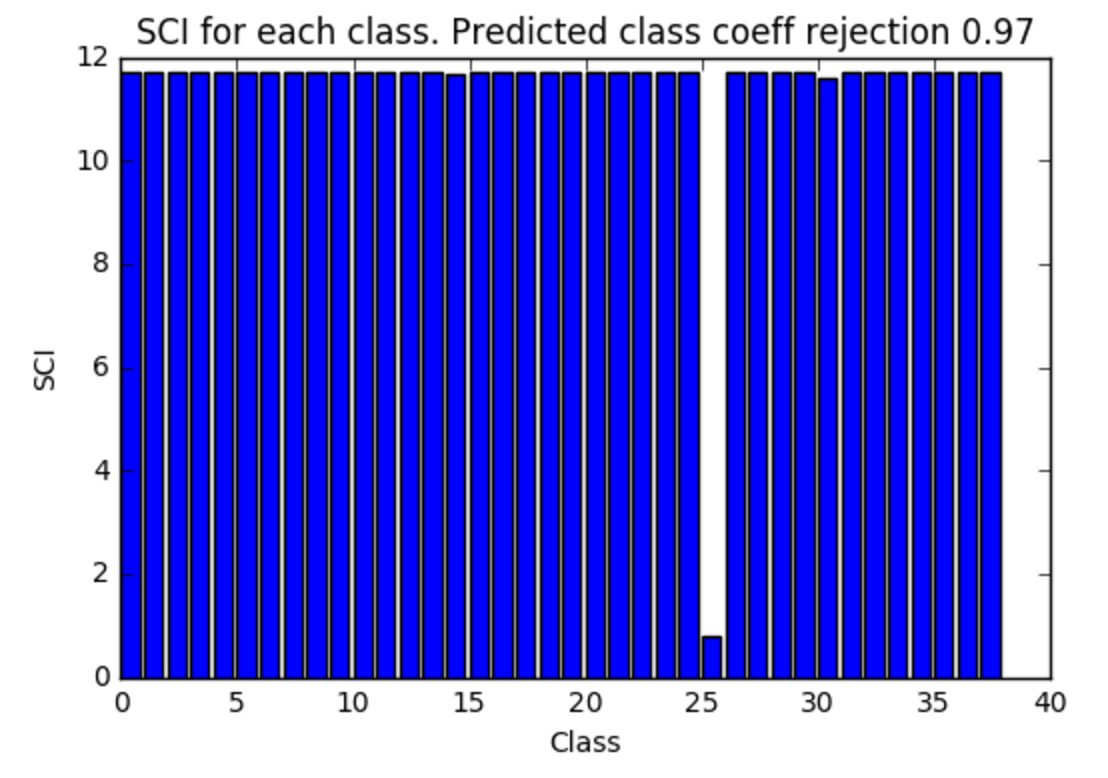
\includegraphics[scale=0.5]{SCI.png}
			\end{center}
			\caption{SCI diagram}
			\label{fa}
			\end{figure}
\end{frame}
%---------------

%---------------

\begin{frame}
\frametitle{Face recognition : our example}

			\begin{figure}[!ht]
			\begin{center}
			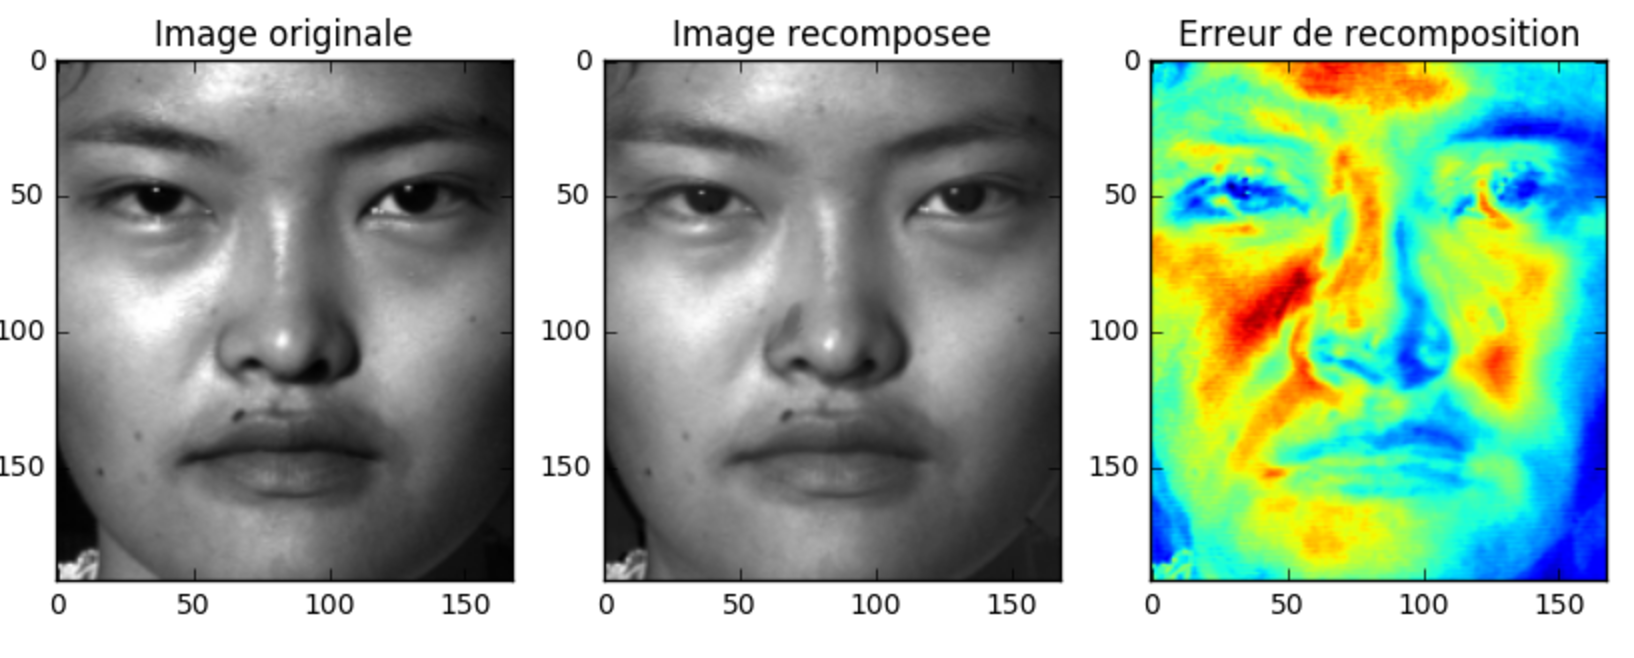
\includegraphics[scale=0.4]{recomposition.png}
			\end{center}
			\caption{Face recomposition}
			\label{fa}
			\end{figure}
\end{frame}

%---------------


\subsection{Extended problem with noise}


\begin{frame}

		\frametitle{Algorithm 2: SRC with noise (relaxed problem)}		

\begin{itemize}			
\item Since the real data are noisy we can rewrite the model : 
$$ y=Ax_{0}+z$$
where $z \in  \mathbb{R}^{m}$ is a noise term with bounded energy, i.e, $\|z\|_{2}< \epsilon$
\item The sparse solution $x_{0}$ can still be approximately recovered by solving the stable $L^{1}$ minimization problem (eq to LASSO) :
$$ \hat{x_{1}}= \argmin \|x\|_{1}  \mbox{ subject to } \|Ax-y\|_{2} \leq \epsilon $$
\end{itemize}
\end{frame}

%---------------

\begin{frame}
\frametitle{Face recognition : our example}

			\begin{figure}[!ht]
			\begin{center}
			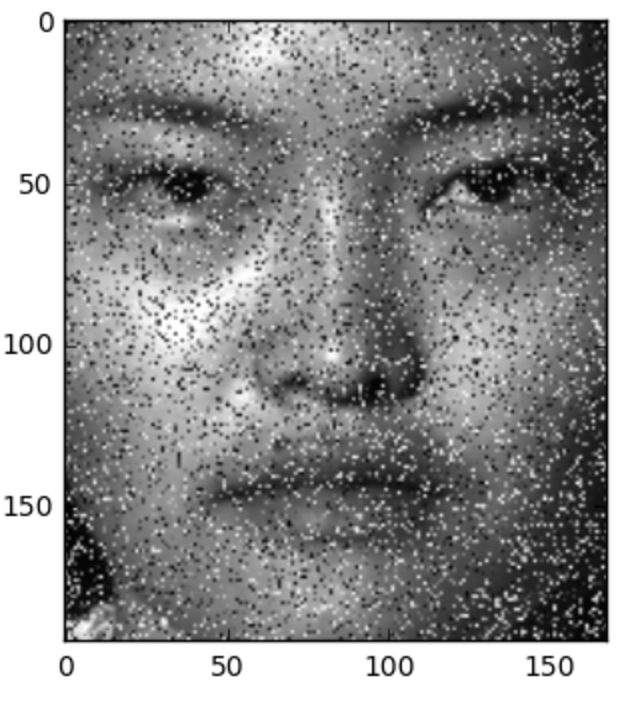
\includegraphics[scale=0.4]{noisy_face.png}
			\end{center}
			\caption{Noisy image}
			\label{fa}
			\end{figure}
\end{frame}

%---------------

\subsection{Extended problem with feature extraction}


\begin{frame}

		\frametitle{Algorithm 3: SRC with feature extraction}		

\begin{itemize}			
\item The feature extraction is crucial because it reduce data dimension and computational cost
\item Most feature transformation involve only linear operations into a \textbf{feature space} represented by $R \in \mathbb{R}^{d \times m}$ with $d <<m$ 
\item The first problem becomes $$\widetilde{y}=Ry=RAx_{0} \in \mathbb{R}^{d}$$
\item The main  results is if $x_{0}$ is \textbf{sparse enough} then with overwhelming probability it can be recovered via $L^{1}$ minimization
\item Random features can be used ! (extremely efficient to generate)
\end{itemize}

\end{frame}

%---------------

\begin{frame}
\frametitle{Face recognition : our example}

			\begin{figure}[!ht]
			\begin{center}
			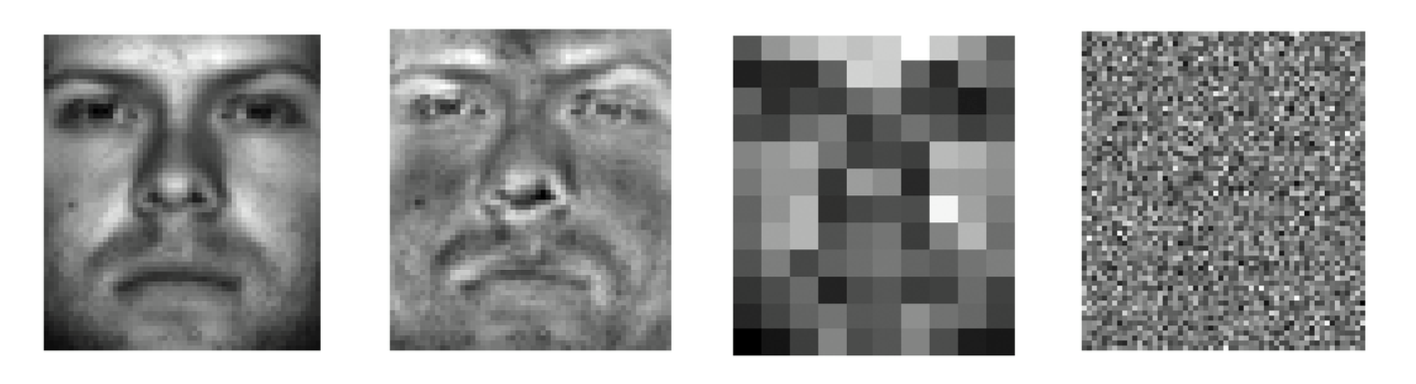
\includegraphics[scale=0.2]{feature_reduc.png}
			\end{center}
			\caption{Feature extraction}
			\label{fa}
			\end{figure}
\end{frame}

%---------------

\subsection{Extended problem with occlusion}


\begin{frame}

		\frametitle{Algorithm 4: SRC with occlusion}		

\begin{itemize}

\item Some corrupted pixels (in a small portion of the image)
\item The problem becomes $y=y_{o}+e_{0}$ where $e_{0} \in \mathbb{R}^{m}$ is a vector of errors (a fraction $\rho$ of its entries are nonzero where pixels are corrupted). 
\item So we can rewrite the roblem as : $$y = \lbrack A,I \rbrack 
\begin{bmatrix}
           x_{0} \\
           e_{0} 
\end{bmatrix}=Bw_{0}$$

\item If the occlusion e covers less than 50 \% of the image the sparsest solution to $y=Bw$ is the true generator $w_{0}=\lbrack x_{0},e_{0} \rbrack $


\end{itemize}

\end{frame}

%---------------

\begin{frame}
\frametitle{Face recognition : our example}

			\begin{figure}[!ht]
			\begin{center}
			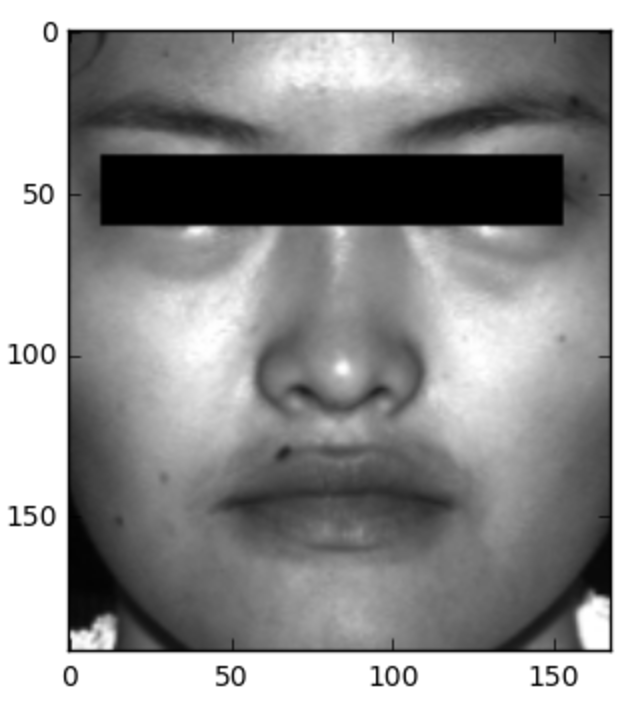
\includegraphics[scale=0.4]{occluded_face.png}
			\end{center}
			\caption{Occluded image}
			\label{fa}
			\end{figure}
\end{frame}

%------------------------------------------------
%------------------------------------------------
\section{Implementation}


\begin{frame}

		\frametitle{What did we do}
		
		\begin{itemize}
		\item Implemented sparse representation algorithm 2 (relaxed version) with LASSO
		\item Applied the algorithm for the situation with noise, occlusion and with different features extractions on Yale Database
		\item Find best $\lambda$ for LASSO with cross val
		\item Ilustrate and compare the algorithm with PCA + SVM approach.
		
		\end{itemize}
		
		
\end{frame}
		

%------------------------------------------------

\begin{frame}

		\frametitle{Performances}



			\begin{figure}[!ht]
			\begin{center}
			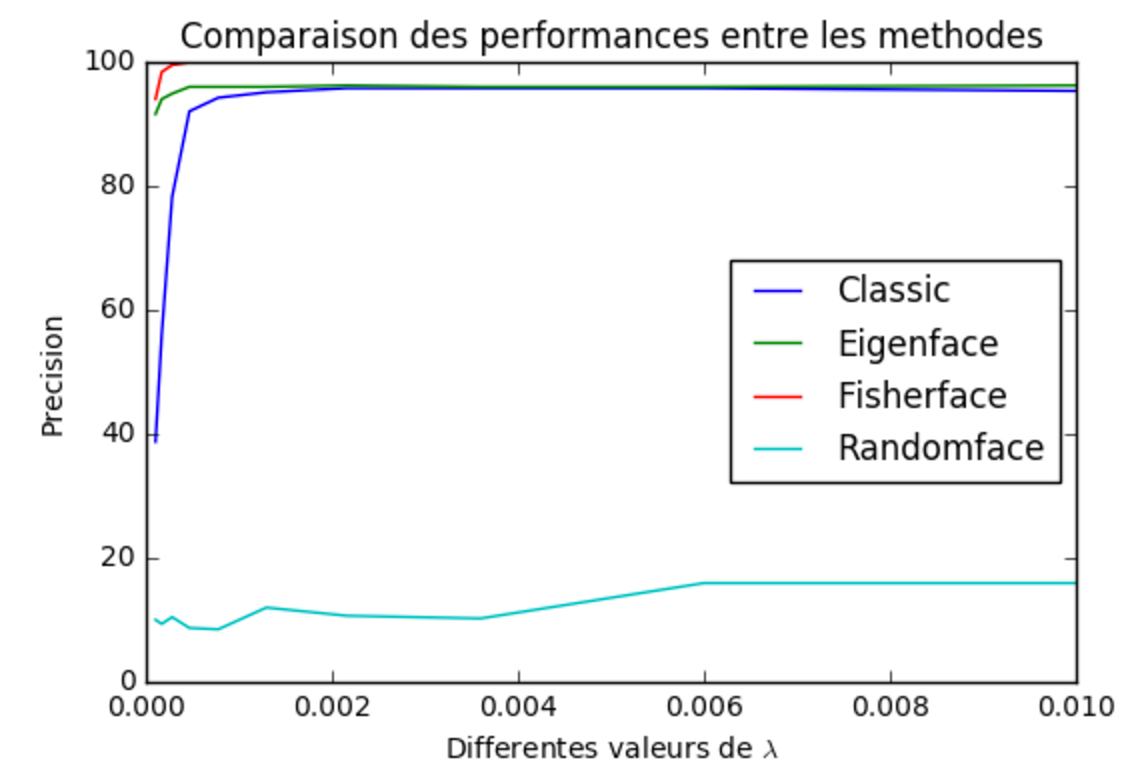
\includegraphics[scale=0.25]{perf1.png}
			\end{center}
			\caption{Occluded image}
			\label{fa}
			\end{figure}
	
		
\end{frame}
		
		%------------------------------------------------

\begin{frame}

		\frametitle{Performances}



			\begin{figure}[!ht]
			\begin{center}
			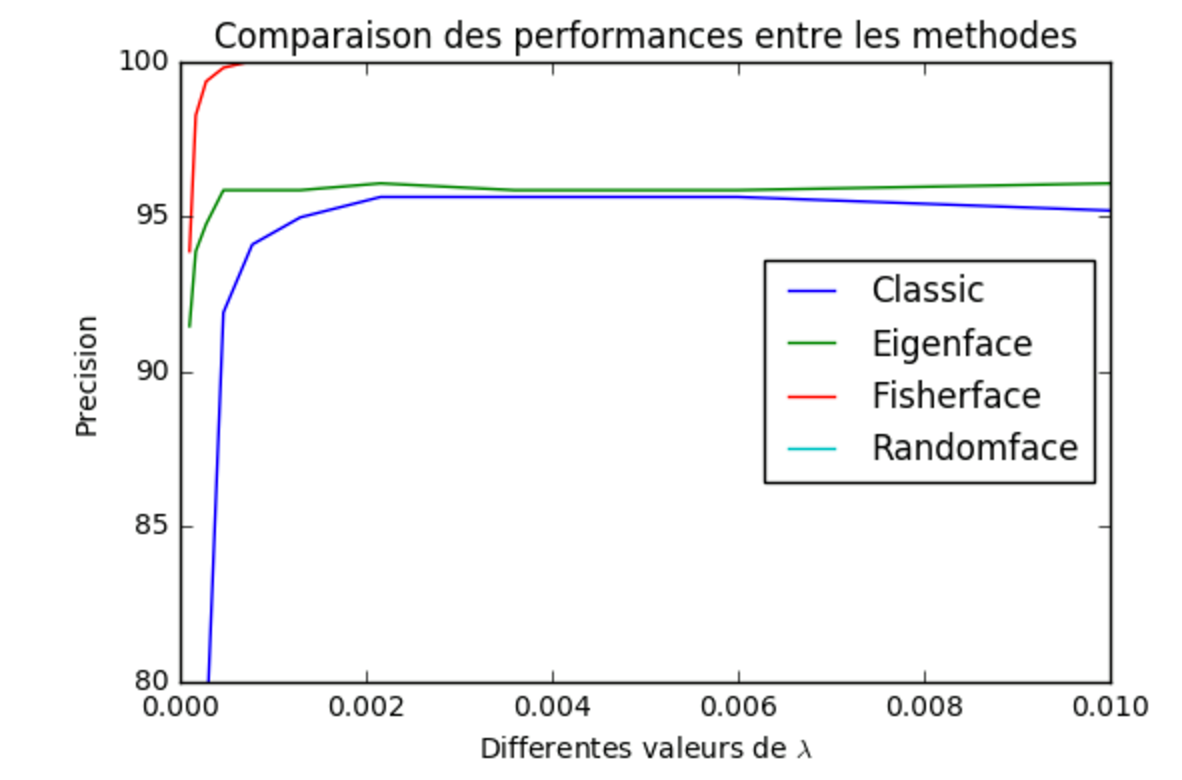
\includegraphics[scale=0.25]{perf2.png}
			\end{center}
			\caption{Occluded image}
			\label{fa}
			\end{figure}
	
		
\end{frame}
%------------------------------------------------




%------------------------------------------------


\end{document}